\documentclass[10pt,a4paper,twocolumn]{article}
% --- 极简中文支持（pdfLaTeX 直接兼容，无需切换编译器）---
\usepackage{CJKutf8} % pdfLaTeX 下最可靠的中文支持

% --- 基础宏包（清理冗余，确保无冲突）---
\usepackage{amsmath, amsfonts, amssymb}
\usepackage{graphicx}
\usepackage{geometry}
\geometry{a4paper,left=2cm,right=2cm,top=2cm,bottom=2cm}
\usepackage{listings}
\usepackage{xcolor}
\usepackage{hyperref}
\usepackage{booktabs}
\usepackage{caption}
\captionsetup{font=small,labelfont=small,skip=0pt}
\usepackage{float}
\setlength{\intextsep}{0pt}
\setlength{\textfloatsep}{0pt}
\usepackage{subcaption}
\captionsetup{subfigure}{skip=0pt}
\usepackage{multirow}
\setlength{\medskipamount}{0pt}
\setlength{\bigskipamount}{0pt}
\setlength{\smallskipamount}{0pt}
\usepackage{algorithm}
\usepackage{algorithmic}
\usepackage{tcolorbox}
\tcbuselibrary{listings,skins}

% 代码块样式设置
\lstset{
    basicstyle=\ttfamily\footnotesize,
    keywordstyle=\color{blue}\bfseries,
    commentstyle=\color{green!60!black},
    stringstyle=\color{orange},
    breaklines=true,
    frame=single,
    frameround=tttt,
    backgroundcolor=\color{gray!10},
    numbers=left,
    numberstyle=\tiny\color{gray},
    xleftmargin=1em,
    framexleftmargin=1em,
    showstringspaces=false,
    aboveskip=2pt,
    belowskip=2pt
}

% 图片相对路径（本次作业图片存放在 teach/pic7 下）
\graphicspath{{pic7/}}

% 段落和间隔设置
\setlength{\parskip}{2pt}
\setlength{\parsep}{0pt}
\setlength{\topsep}{2pt}
\setlength{\itemsep}{2pt}

% 数学符号宏定义
\newcommand{\fro}[1]{\left\|#1\right\|_F}
\newcommand{\tr}{\mathrm{tr'}}
\newcommand{\argmin}{\mathop{\mathrm{argmin}}}
\newcommand{\R}{\mathbb{R}}

\title{光栅化与光路追踪实验}
\author{宁尚哲 \quad PB24000099}
\date{\today}

\begin{document}
\begin{CJK*}{UTF8}{gbsn}
\maketitle

\begin{abstract}

\end{abstract}

\section{引言}
本实验实现了基于光栅化与光线追踪的实时渲染系统，涵盖了Blinn-Phong光照模型、阴影映射、屏幕空间环境光遮蔽（SSAO）、百分比接近软阴影（PCSS）以及路径追踪中的矩形光源采样、Russian Roulette终止策略和多重重要性采样（MIS）等技术。实验通过对比光栅化与光线追踪两种渲染方法，深入探讨了不同算法在真实感渲染中的性能与质量权衡。

\section{光栅化部分}

\subsection{基础Blinn-Phong光照与着色模型}
\subsubsection{数学公式与原理}
Blinn-Phong模型是实时渲染中广泛采用的光照近似方法，通过组合环境光、漫反射和镜面反射三个分量来模拟物体表面的光照效果。设表面法线为 $\mathbf{n}$，入射光方向为 $\mathbf{l}$，观察方向为 $\mathbf{v}$，半程向量定义为 $\mathbf{h}=\frac{\mathbf{l}+\mathbf{v}}{\|\mathbf{l}+\mathbf{v}\|}$。光照模型可表示为：
$
L_o = L_{ambient} + L_{diffuse} + L_{specular}
$
其中各分量计算如下：
$
L_{ambient} = k_a \cdot I_{ambient}
$
$
L_{diffuse} = k_d \cdot I_{light} \cdot \max(0, \mathbf{n} \cdot \mathbf{l})
$
$
L_{specular} = k_s \cdot I_{light} \cdot \max(0, \mathbf{n} \cdot \mathbf{h})^{\alpha}
$
这里 $k_a, k_d, k_s$ 分别为环境光、漫反射和镜面反射系数，$\alpha$ 为高光指数，控制高光的聚焦程度。

法线贴图技术通过在切线空间中存储扰动后的法线信息来增强表面细节。设切线空间法线为 $\mathbf{n}_{tangent}$，通过TBN矩阵变换到世界空间：
$
\mathbf{n}_{world} = \mathbf{T} \cdot \mathbf{n}_{tangent}
$
其中 $\mathbf{T} = [\mathbf{t}, \mathbf{b}, \mathbf{n}]$ 为由切线、副切线和法线构成的变换矩阵。
\subsubsection{代码实现}
实现采用延迟渲染架构，将几何信息渲染到G-Buffer中，然后在屏幕空间进行光照计算。G-Buffer生成阶段主要完成法线贴图的解码与TBN矩阵构建。由于模型未提供显式切线数据，采用屏幕空间导数方法动态计算切线向量：
\begin{lstlisting}[language=GLSL, caption={Tangent calculation for TBN matrix construction}]
vec3 edge1 = dFdx(vertexPosition);
vec3 edge2 = dFdy(vertexPosition);
vec2 deltaUV1 = dFdx(vTexcoord);
vec2 deltaUV2 = dFdy(vTexcoord);
vec3 tangent = edge1 * deltaUV2.y - edge2 * deltaUV1.y;
\end{lstlisting}
通过Gram-Schmidt正交化确保切线与法线垂直，然后构建TBN矩阵将切线空间法线变换到世界空间。

在延迟光照阶段，从G-Buffer读取位置、法线、反照率和粗糙度信息，计算Blinn-Phong光照。高光指数通过粗糙度参数映射：
\begin{lstlisting}[language=GLSL, caption={Blinn-Phong specular calculation}]
float shininess = (1.0 - roughness) * 128.0;
float spec = pow(max(dot(normal, halfDir), 0.0), shininess);
\end{lstlisting}
\subsubsection{实验效果验证}
\begin{figure}[H]
\centering
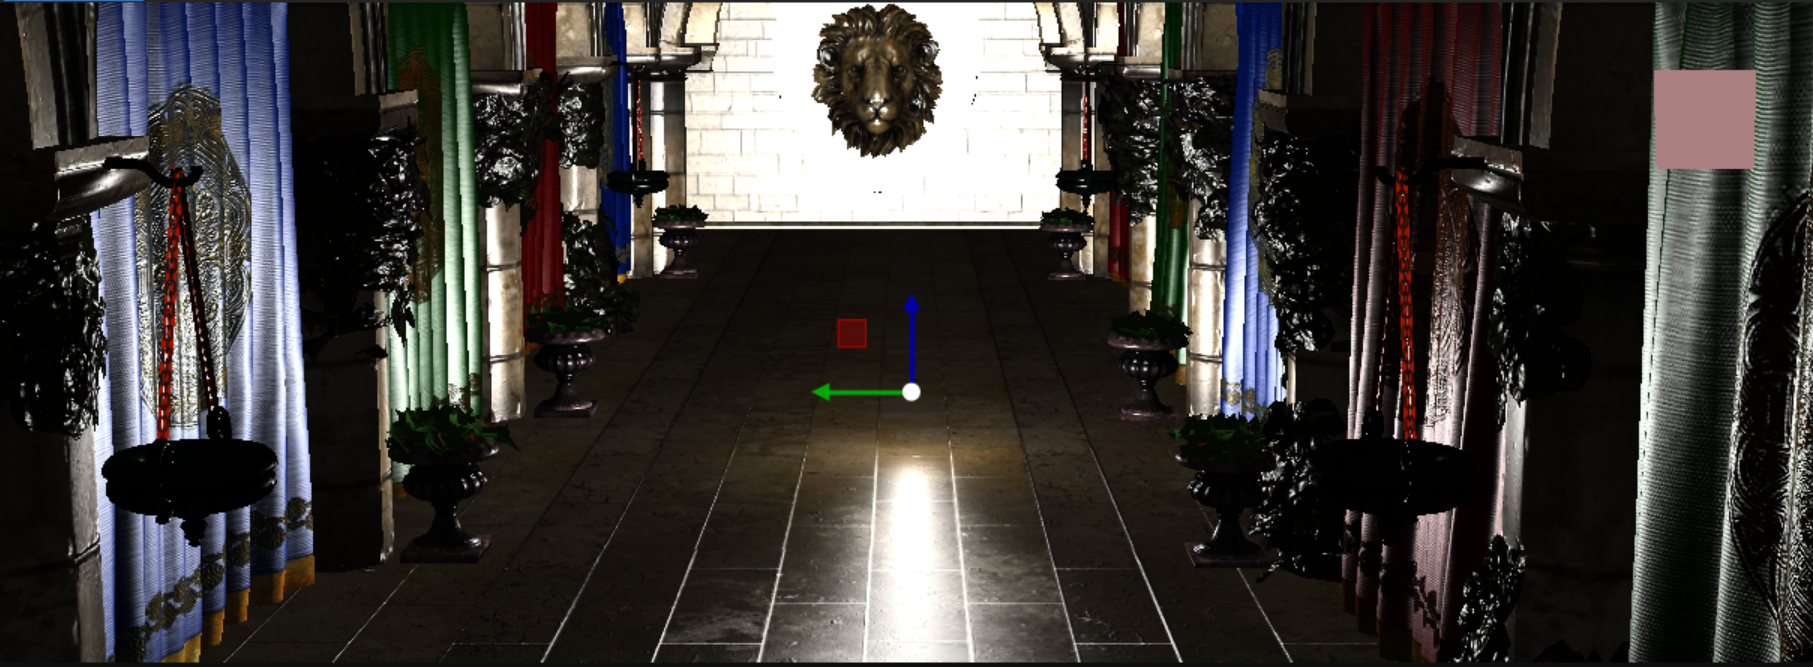
\includegraphics[width=0.45\textwidth]{image-20260422225642258.png}
\caption{G-Buffer导入场景验证图}
\end{figure}

\subsection{Shadow Mapping}
\subsubsection{数学公式与原理}
阴影映射算法通过从光源视角渲染深度图来检测遮挡关系。设光源视图矩阵为 $\mathbf{V}_l$，投影矩阵为 $\mathbf{P}_l$，则光空间变换矩阵为 $\mathbf{M}_l = \mathbf{P}_l \mathbf{V}_l$。对于世界空间点 $\mathbf{p}_w$，其在光空间的齐次坐标为：
$
\mathbf{p}_l = \mathbf{M}_l \begin{bmatrix} \mathbf{p}_w \\ 1 \end{bmatrix}
$
经过透视除法得到NDC坐标，深度值为 $z_l = p_{l,z} / p_{l,w}$。阴影测试通过比较当前深度与阴影贴图中的深度值实现：
$
S(\mathbf{p}) = \begin{cases} 0 & \text{if } z_l > z_{tex} + \epsilon \\ 1 & \text{otherwise} \end{cases}
$
其中 $\epsilon$ 为偏置项，用于避免阴影痤疮（shadow acne）伪影。
\subsubsection{代码实现}
阴影映射实现包含深度图生成和阴影测试两个阶段。在深度图生成阶段，顶点着色器将顶点变换到光空间，片元着色器输出归一化深度值：
\begin{lstlisting}[language=GLSL, caption={Shadow depth map generation}]
vec4 clipPos = light_projection * light_view * vec4(vertexPosition, 1.0);
float ndcDepth = clipPos.z / clipPos.w;
shadow_map0 = ndcDepth * 0.5 + 0.5;
\end{lstlisting}
在光照计算阶段，将当前像素的世界坐标变换到光空间，采样阴影贴图并比较深度值：
\begin{lstlisting}[language=GLSL, caption={Shadow test implementation}]
vec4 lightSpacePos = lights[i].light_projection * lights[i].light_view * vec4(pos, 1.0);
vec3 lightSpaceNDC = lightSpacePos.xyz / lightSpacePos.w;
vec2 shadowUV = lightSpaceNDC.xy * 0.5 + 0.5;
float currentDepth = lightSpaceNDC.z * 0.5 + 0.5;
float shadowDepth = texture(shadow_maps, vec3(shadowUV, layer)).x;
float shadowFactor = (currentDepth > shadowDepth + 0.005) ? 0.0 : 1.0;
\end{lstlisting}
\subsubsection{实验效果验证}
\begin{figure}[H]
\centering
\begin{subfigure}{0.32\textwidth}
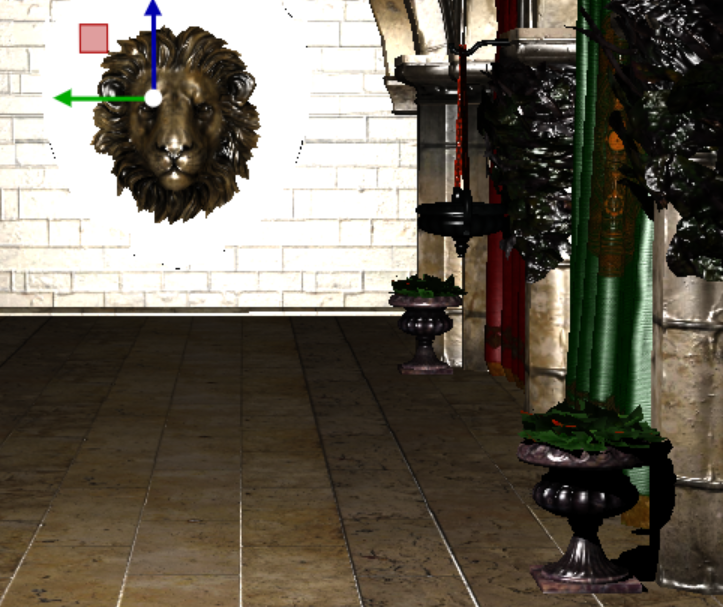
\includegraphics[width=\textwidth]{image-20260422234219210.png}
\caption{硬阴影效果}
\end{subfigure}
\begin{subfigure}{0.32\textwidth}
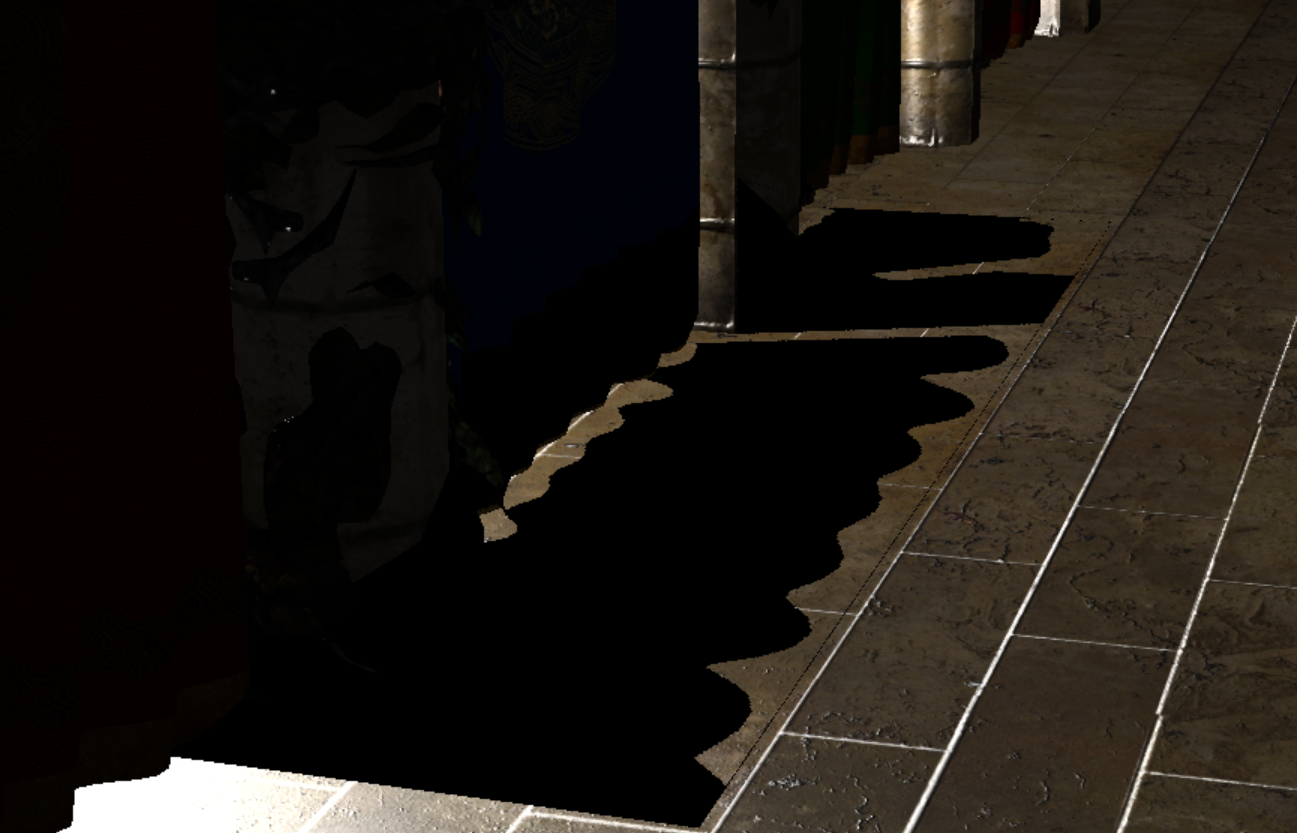
\includegraphics[width=\textwidth]{image-20260423161125771.png}
\caption{窗帘阴影}
\end{subfigure}
\begin{subfigure}{0.32\textwidth}
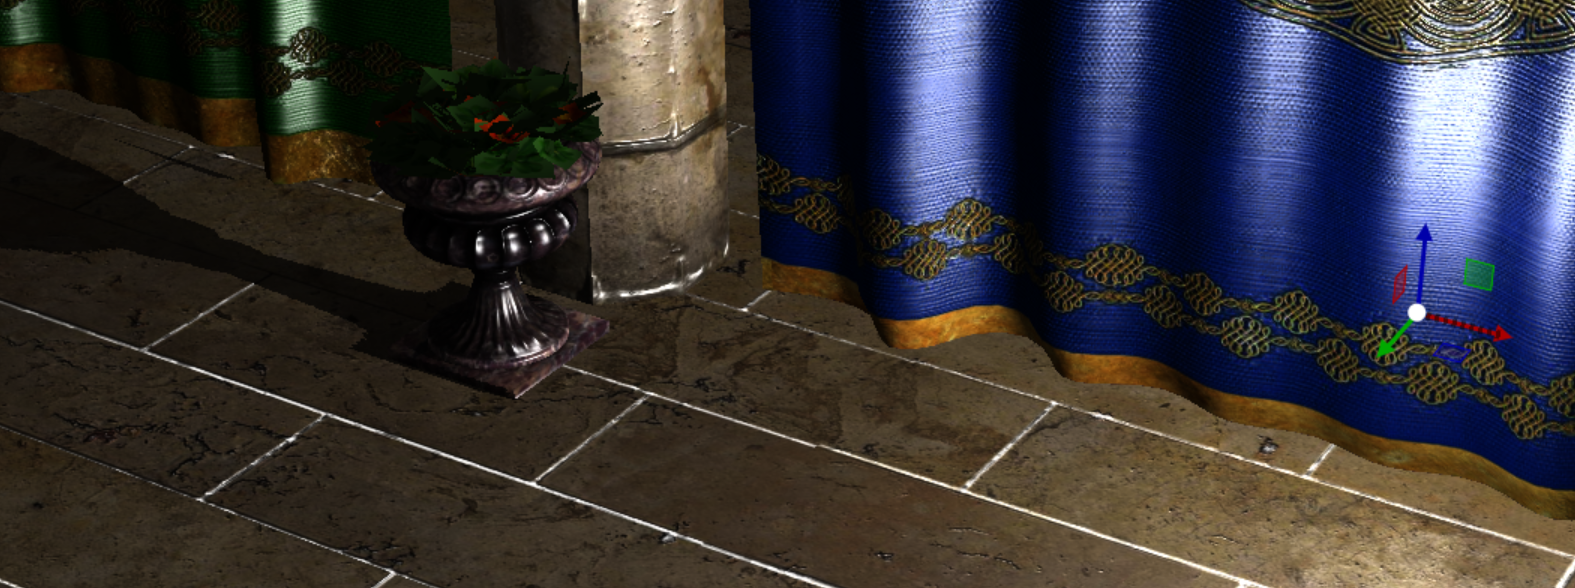
\includegraphics[width=\textwidth]{image-20260423162313598.png}
\caption{狭长阴影}
\end{subfigure}
\caption{Shadow Mapping硬阴影效果}
\end{figure}

\begin{figure}[H]
\centering
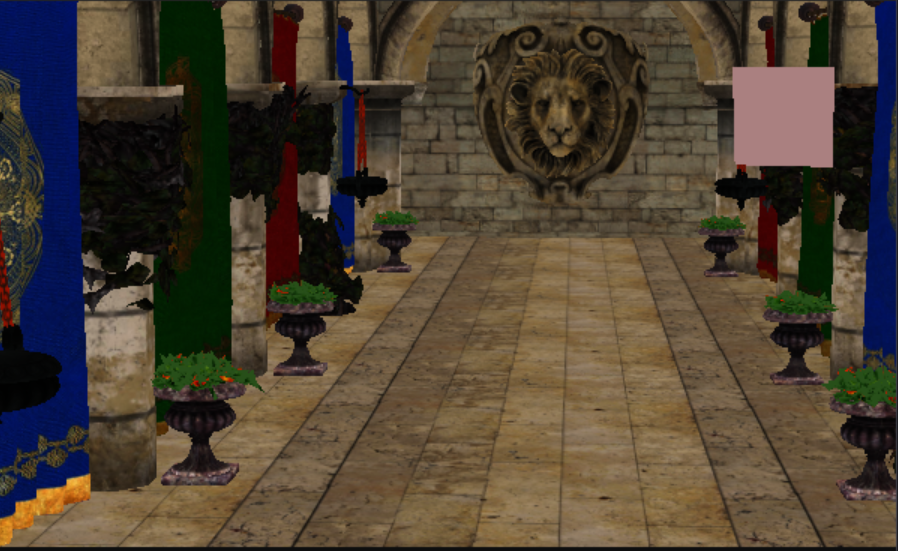
\includegraphics[width=0.4\textwidth]{image-20260424225243844.png}
\caption{环境光照效果}
\end{figure}

\subsection{PCSS(Rast Optional)}
\subsubsection{数学公式与原理}
百分比接近软阴影（PCSS）通过模拟面积光源的半影效应产生柔和的阴影边缘。算法分为三个步骤：首先在接收点周围搜索遮挡物，计算平均遮挡深度 $\bar{z}_b$；然后根据相似三角形原理估计半影半径：
$
w_{penumbra} = \frac{d_{receiver} - \bar{z}_b}{\bar{z}_b} \cdot w_{light}
$
其中 $d_{receiver}$ 为接收点到光源的距离，$w_{light}$ 为光源尺寸；最后在估计的半影半径内进行百分比接近滤波（PCF），计算软阴影因子。
\subsubsection{代码实现}
PCSS实现使用Poisson盘采样来减少噪声并提高采样效率。遮挡物搜索函数在给定半径内采样深度贴图：
\begin{lstlisting}[language=GLSL, caption={PCSS blocker search function}]
float findBlockerAvgDepth(sampler2DArray sm, vec2 uv, float receiverDepth, 
    int layer, float searchRadiusUV) {
    int blockers = 0;
    float avg = 0.0;
    for (int i = 0; i < PCSS_BLOCKER_SAMPLES; ++i) {
        vec2 offset = poissonDisk[i] * searchRadiusUV;
        float d = texture(sm, vec3(uv + offset, layer)).r;
        if (d + SHADOW_BIAS < receiverDepth) {
            avg += d;
            blockers++;
        }
    }
    return (blockers == 0) ? -1.0 : avg / float(blockers);
}
\end{lstlisting}
主PCSS函数根据遮挡物平均深度估计半影大小，并在该半径内执行PCF滤波：
\begin{lstlisting}[language=GLSL, caption={PCSS main function implementation}]
float computePCSS(sampler2DArray sm, vec2 uv, float receiverDepth, 
int layer, float lightRadius) {
    float avgBlocker = findBlockerAvgDepth(sm, uv, receiverDepth, layer, 0.01);
    if (avgBlocker < 0.0) return 1.0;
    float penumbra = (receiverDepth - avgBlocker) / max(avgBlocker, 1e-6) * lightRadius;
    float radiusUV = clamp(penumbra, PCSS_MIN_RADIUS_UV, PCSS_MAX_RADIUS_UV);
    return pcfFilter(sm, uv, receiverDepth, layer, radiusUV);
}
\end{lstlisting}
\subsubsection{实验效果验证}
\begin{figure}[H]
\centering
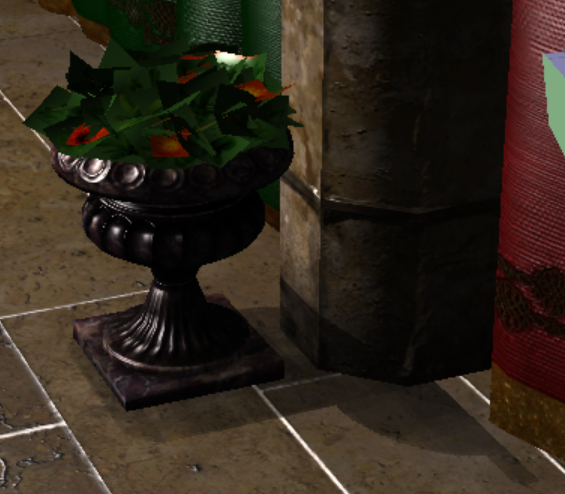
\includegraphics[width=0.5\textwidth]{image-20260423224933234.png}
\caption{PCSS软阴影效果}
\end{figure}

\subsection{SSAO(Rast Optional)}
\subsubsection{数学公式与原理}
屏幕空间环境光遮蔽（SSAO）通过在屏幕空间中采样邻域像素的深度信息来近似计算环境光遮蔽。对于每个像素，在其法线方向的半球内采样多个点，比较采样点与场景中实际几何体的深度关系。遮蔽因子计算为：
$AO(\mathbf{p}) = 1 - \frac{1}{N} \sum_{i=1}^{N} V(\mathbf{p}, \mathbf{p} + \mathbf{r}_i) \cdot w(\|\mathbf{r}_i\|)
$
其中 $V(\cdot)$ 为可见性函数，当采样点被遮挡时返回1，否则返回0；$w(\cdot)$ 为距离权重函数，通常采用线性衰减；$\mathbf{r}_i$ 为在切线空间中的采样方向。
\subsubsection{代码实现}
SSAO实现首先在CPU端生成采样核和旋转噪声纹理。采样核使用半球采样并按距离加权：
\begin{lstlisting}[language=C++, caption={SSAO sampling kernel generation}]
for (unsigned int i = 0; i < kernelSize; ++i) {
    glm::vec3 sample(randomFloats(generator) * 2.0 - 1.0,
                    randomFloats(generator) * 2.0 - 1.0,
                    randomFloats(generator));
    sample = glm::normalize(sample);
    sample *= randomFloats(generator);
    float scale = float(i) / float(kernelSize);
    scale = 0.1f + 0.9f * (scale * scale);
    sample *= scale;
    ssaoKernel.push_back(sample);
}
\end{lstlisting}
在着色器中，构建TBN矩阵将采样方向变换到视图空间，然后对每个采样点进行深度比较：
\begin{lstlisting}[language=GLSL, caption={SSAO depth comparison implementation}]
vec3 sampleView = fragPosView + TBN * samples[i] * radius;
vec4 offset = projection * vec4(sampleView, 1.0);
offset.xyz /= offset.w;
vec2 sampleUV = offset.xy * 0.5 + 0.5;
float rangeCheck = smoothstep(0.0, 1.0, radius / max(0.0001, length(fragPosView - sampleViewFromTex)));
if (sampleViewFromTex.z >= sampleView.z + bias)
    occlusion += rangeCheck;
\end{lstlisting}
\subsubsection{实验效果验证}
\begin{figure}[H]
\centering
\begin{subfigure}{0.48\textwidth}
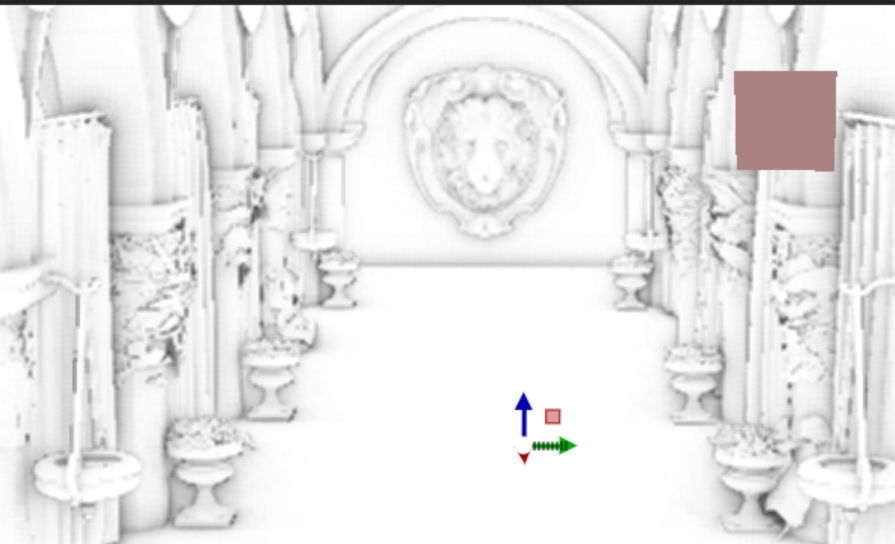
\includegraphics[width=\textwidth]{image-20260424230114565.png}
\caption{SSAO原始效果}
\end{subfigure}
\begin{subfigure}{0.48\textwidth}
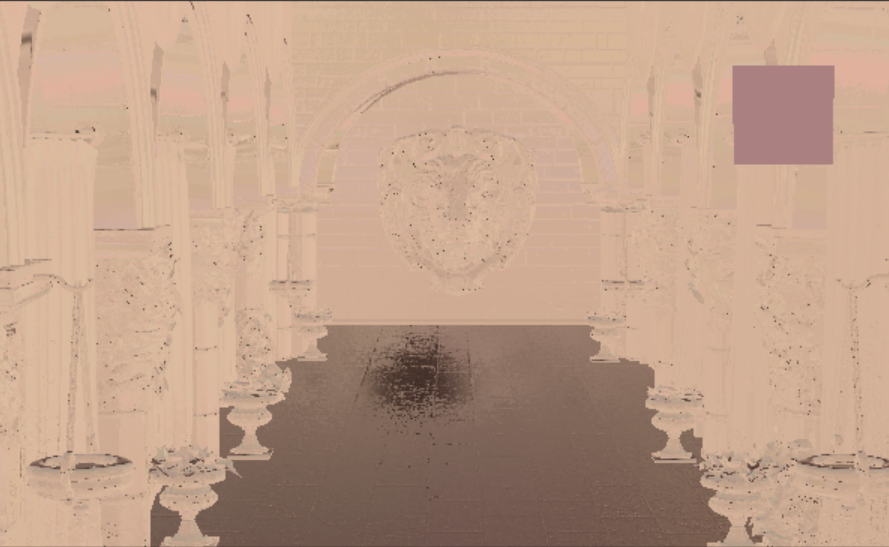
\includegraphics[width=\textwidth]{image-20260424230806932.png}
\caption{SSAO Transfer效果}
\end{subfigure}
\caption{SSAO环境光遮蔽效果}
\end{figure}

\begin{figure}[H]
\centering
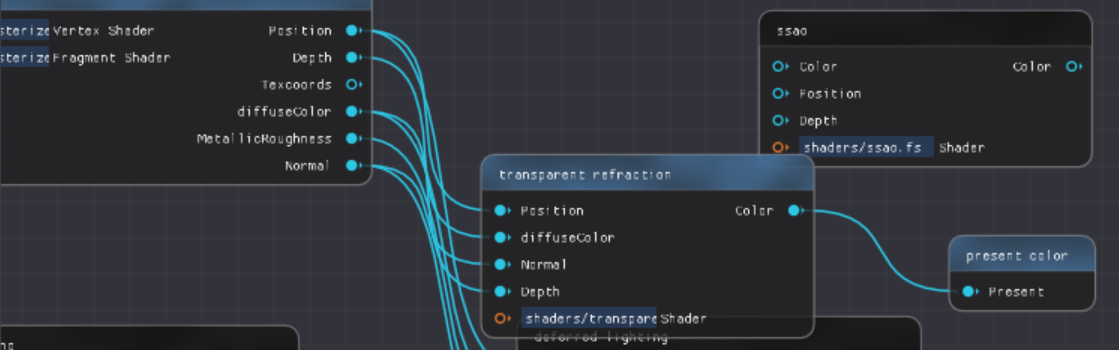
\includegraphics[width=0.4\textwidth]{image-20260424230822602.png}
\caption{SSAO节点连线图}
\end{figure}

\subsection{Displacement Mapping(Rast Optional)}
\subsubsection{数学公式与原理}
位移贴图技术通过纹理值直接修改顶点位置，在几何层面产生真实的凹凸效果，与仅改变光照的法线贴图不同。设原始顶点位置为 $\mathbf{p}$，法线为 $\mathbf{n}$，位移贴图采样值为 $d(\mathbf{u})$，则修正后的顶点位置为：
$
\mathbf{p}' = \mathbf{p} + (s \cdot d(\mathbf{u}) + b) \cdot \mathbf{n}
$
其中 $s$ 为位移缩放因子，$b$ 为偏置量。位移贴图通常需要配合几何细分才能获得高质量的细节表现。
\subsubsection{代码实现}
位移贴图在顶点着色器中实现，首先采样位移贴图获取位移值，然后沿法线方向偏移顶点位置：
\begin{lstlisting}[language=GLSL, caption={Displacement mapping vertex offset implementation}]
float displacement = texture(displacementSampler, vTexcoord).r;
vec3 displacedPosition = vertexPosition + normal * (displacementScale * displacement + displacementBias);
\end{lstlisting}
由于位移会改变几何形状，需要在位移后重新计算法线或使用更高精度的细分来保证光照正确性。
\subsubsection{实验效果验证}
\begin{figure}[H]
\centering
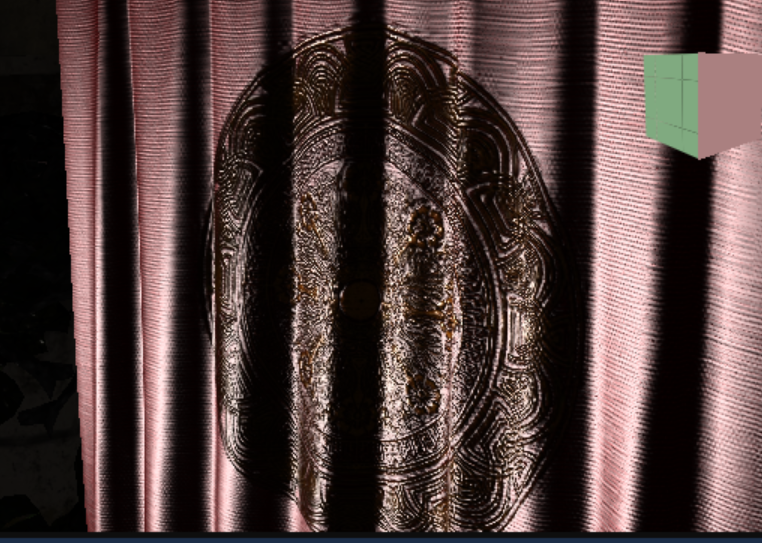
\includegraphics[width=0.5\textwidth]{image-20260424232331942.png}
\caption{位移贴图效果}
\end{figure}

\begin{figure}[H]
\centering
\begin{subfigure}{0.48\textwidth}
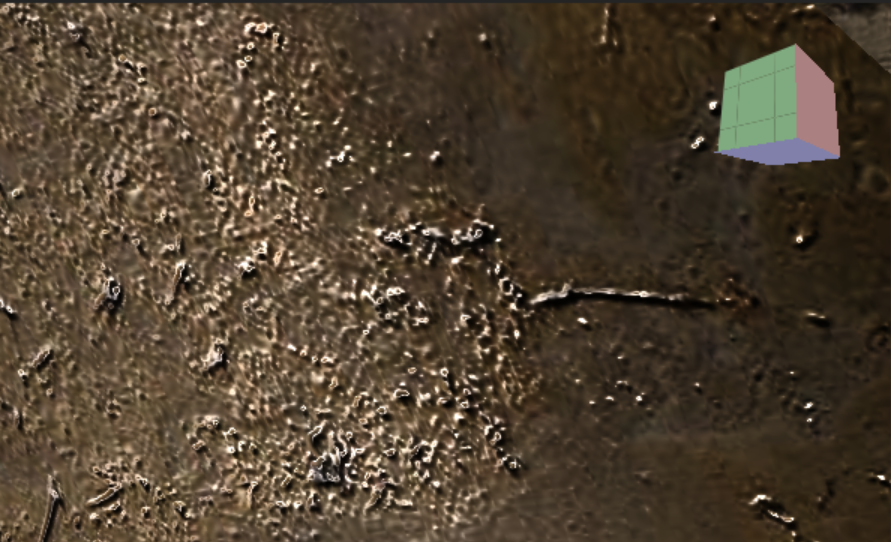
\includegraphics[width=\textwidth]{image-20260424233416738.png}
\caption{纹理凹陷验证}
\end{subfigure}
\begin{subfigure}{0.48\textwidth}
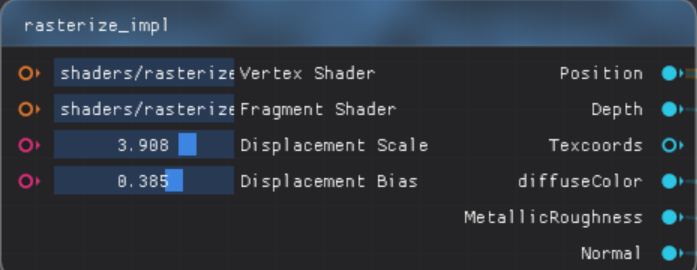
\includegraphics[width=\textwidth]{image-20260424233438016.png}
\caption{位移参数节点暴露}
\end{subfigure}
\caption{位移贴图参数验证}
\end{figure}

\section{光线追踪部分}
\subsection{矩形光源}
\subsubsection{数学公式与原理}
矩形光源作为面积光源，其直接光照贡献需要通过对光源表面积分来计算。设矩形由四个角点 $\mathbf{c}_0, \mathbf{c}_1, \mathbf{c}_2, \mathbf{c}_3$ 定义，面积为 $A$，光源自发光为 $L_e$。对于表面点 $\mathbf{x}$，矩形光源的直接光照贡献为：
$
L_{direct}(\mathbf{x}) = \int_A L_e(\mathbf{y}) f_r(\mathbf{x}, \omega_i, \omega_o) \frac{|\cos\theta_x| |\cos\theta_y|}{\|\mathbf{y} - \mathbf{x}\|^2} dA_y
$
其中 $\mathbf{y}$ 为光源表面上的点，$\theta_x$ 为入射光线与表面法线的夹角，$\theta_y$ 为出射光线与光源面法线的夹角，$f_r$ 为BRDF函数。

采用蒙特卡洛积分方法，通过对光源表面均匀采样来估计上述积分。均匀采样的概率密度函数（PDF）在面积测度下为 $p_A(\mathbf{y}) = 1/A$，转换到立体角测度下为：
$
p_{\Omega}(\omega_i) = \frac{\|\mathbf{y} - \mathbf{x}\|^2}{A |\cos\theta_y|}
$ 
\subsubsection{代码实现}
矩形光源的采样采用双线性插值在矩形表面生成均匀分布的采样点：
\begin{lstlisting}[language=C++, caption={Rectangular light uniform sampling}]
float u = uniform_float();
float v = uniform_float();
GfVec3f sampledPos = (1 - u) * (1 - v) * corner0 + 
                     (1 - u) * v * corner1 + 
                     u * (1 - v) * corner2 + 
                     u * v * corner3;
\end{lstlisting}
采样方向和PDF计算如下：
\begin{lstlisting}[language=C++, caption={Rectangular light PDF calculation}]
dir = (sampledPos - pos).GetNormalized();
GfVec3f edge1 = corner1 - corner0;
GfVec3f edge2 = corner2 - corner0;
float area = GfCross(edge1, edge2).GetLength();
GfVec3f normal = GfCross(edge1, edge2).GetNormalized();
float cosVal = GfDot(-dir, normal);
float distance = (sampledPos - pos).GetLength();
sample_light_pdf = distance * distance / (area * cosVal);
\end{lstlisting}
相交测试通过射线与平面的交点计算，然后验证交点是否在矩形范围内。
\subsubsection{实验效果验证}
\begin{figure}[H]
\centering
\begin{subfigure}{0.32\textwidth}
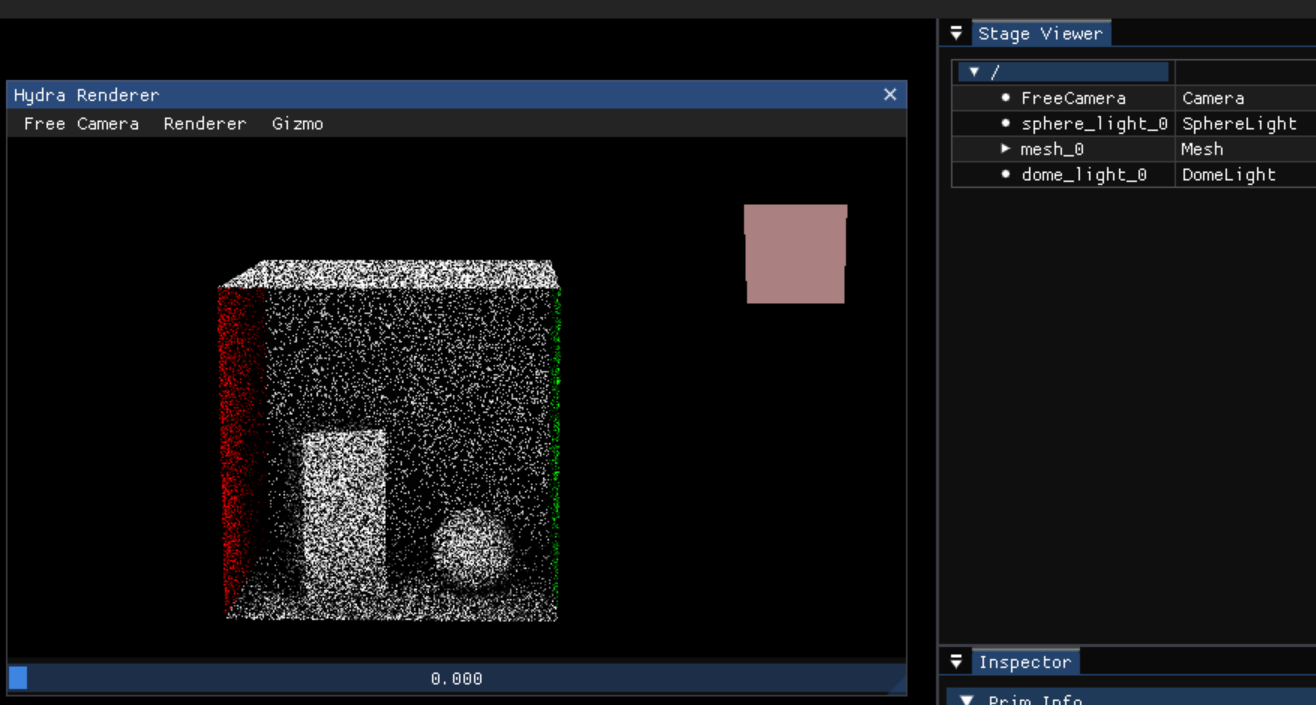
\includegraphics[width=\textwidth]{image-20260423180035981.png}
\caption{基础光照配置}
\end{subfigure}
\begin{subfigure}{0.32\textwidth}
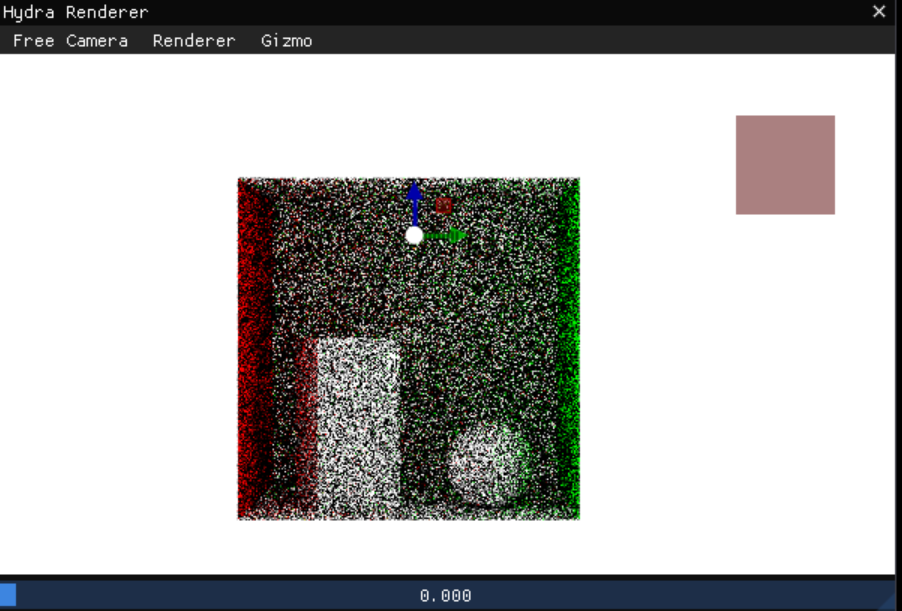
\includegraphics[width=\textwidth]{image-20260423200533181.png}
\caption{基础光追效果}
\end{subfigure}
\begin{subfigure}{0.32\textwidth}
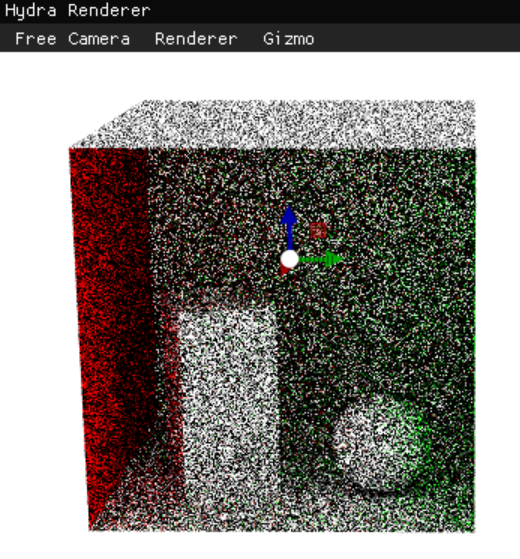
\includegraphics[width=\textwidth]{image-20260423200933092.png}
\caption{上方视角}
\end{subfigure}
\caption{基础光追在康奈尔模型下验证效果}
\end{figure}

\begin{figure}[H]
\centering
\includegraphics[width=0.45\textwidth]{image-20260424235530680.png}
\caption{矩形光源验证效果}
\end{figure}




\subsection{着色递归计算与Russian Roulette轮盘赌}
\subsubsection{数学公式与原理}
路径追踪通过递归求解渲染方程来模拟全局光照效果。渲染方程描述了出射辐射亮度与入射辐射亮度的关系：
$
L_o(\mathbf{x}, \omega_o) = L_e(\mathbf{x}, \omega_o) + \int_{\Omega} f_r(\mathbf{x}, \omega_i, \omega_o) L_i(\mathbf{x}, \omega_i) \cos\theta_i d\omega_i
$
其中 $L_e$ 为自发光项，$f_r$ 为BRDF函数，$\Omega$ 为入射光线的半球方向集合。

采用递归路径追踪时，路径长度随递归深度指数增长，为避免无限递归和计算开销过大，引入Russian Roulette（俄罗斯轮盘赌）终止策略。在递归深度 $d$ 处，以概率 $p_d$ 继续追踪，若继续则将路径贡献除以 $p_d$ 以保持估计的无偏性：
$
L_{indirect} = \frac{1}{p_d} \cdot f_r \cdot L_i \cdot \frac{\cos\theta}{pdf}
$
\subsubsection{代码实现}
路径追踪的递归实现包含直接光照和间接光照两部分。直接光照通过光源采样计算，间接光照通过BRDF采样递归计算：
\begin{lstlisting}[language=C++, caption={Path tracing indirect lighting calculation}]
GfVec3f directLight = EstimateDirectLight(si, uniform_float);

GfVec3f wi;
float brdf_pdf;
auto brdf_val = si.Sample(wi, brdf_pdf, uniform_float);

if (brdf_pdf > 0 && GfDot(wi, si.shadingNormal) > 0) {
    GfRay indirect_ray(si.position + 0.0001f * si.geometricNormal, wi);
    GfVec3f indirect_radiance = EstimateOutGoingRadiance(
        indirect_ray, uniform_float, recursion_depth + 1);
    float cos_theta = GfDot(wi, si.shadingNormal);
    globalLight = GfCompMult(brdf_val, indirect_radiance) * cos_theta / brdf_pdf;
}
\end{lstlisting}
Russian Roulette实现根据递归深度动态调整终止概率：
\begin{lstlisting}[language=C++, caption={Russian Roulette termination strategy implementation}]
if (recursion_depth >= 3) {
    float max_component = std::max({ color[0], color[1], color[2] });
    float continue_prob = std::min(0.95f, max_component);
    
    if (uniform_float() > continue_prob) {
        return directLight;
    }
    color = (directLight + globalLight) / continue_prob;
} else {
    color = directLight + globalLight;
}
\end{lstlisting}
\subsubsection{实验效果验证}

\begin{figure}[H]
\centering
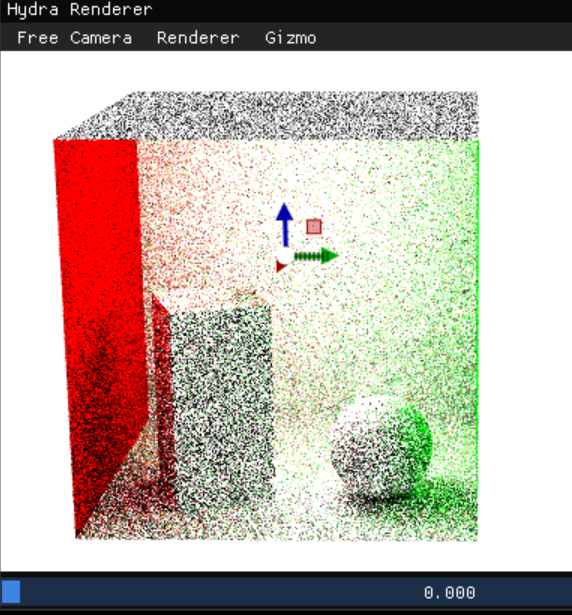
\includegraphics[width=0.45\textwidth]{image-20260423202730458.png}
\caption{调整光强与半径效果}
\end{figure}



\subsection{BRDF模型与MIS}
\subsubsection{数学公式与原理}
本实验实现了基于物理的BRDF模型，结合Lambert漫反射和GGX镜面反射。GGX法线分布函数（NDF）定义为：
$
D_{GGX}(\mathbf{h}) = \frac{\alpha^2}{\pi[(\mathbf{n} \cdot \mathbf{h})^2(\alpha^2 - 1) + 1]^2}
$
其中 $\mathbf{h}$ 为半程向量，$\alpha$ 为粗糙度参数。Fresnel项采用Schlick近似：
$
F(\mathbf{v}, \mathbf{h}) = F_0 + (1 - F_0)(1 - \mathbf{v} \cdot \mathbf{h})^5
$
几何遮蔽函数使用Smith-GGX模型：
$
G(\mathbf{l}, \mathbf{v}, \mathbf{h}) = \frac{2(\mathbf{n} \cdot \mathbf{l})}{\mathbf{n} \cdot \mathbf{l} + \sqrt{\alpha^2 + (1 - \alpha^2)(\mathbf{n} \cdot \mathbf{l})^2}} \cdot \frac{2(\mathbf{n} \cdot \mathbf{v})}{\mathbf{n} \cdot \mathbf{v} + \sqrt{\alpha^2 + (1 - \alpha^2)(\mathbf{n} \cdot \mathbf{v})^2}}
$

BRDF采样采用基于金属度（metallic）的混合策略：
$
p(\omega_i) = (1 - m)p_{diffuse}(\omega_i) + m p_{specular}(\omega_i)
$
其中 $m$ 为金属度参数，控制漫反射和镜面反射的权重。

多重重要性采样（MIS）采用power heuristic合并光源采样和BRDF采样的结果：
$
w = \frac{p_1^2}{p_1^2 + p_2^2}
$
这种加权方法能有效减少方差，提高渲染质量。 
\subsubsection{代码实现}
BRDF采样根据金属度参数选择采样策略：
\begin{lstlisting}[language=C++, caption={BRDF sampling strategy selection}]
if (uniform_float() < metallic) {
    // GGX specular sampling
    auto sampledDir = CosineWeightedDirection(sample2D, sample_pos_pdf);
    // Calculate half vector and reflection direction
} else {
    // Lambert diffuse sampling
    wi = CosineWeightedDirection(sample2D, pdf);
}
\end{lstlisting}
BRDF评估结合漫反射和镜面项：
\begin{lstlisting}[language=C++, caption={BRDF evaluation implementation}]
GfVec3f diffuse = diffuseColor / M_PI;
GfVec3f F = SchlickFresnel(halfDir, viewDir, F0);
float D = GGXDistribution(normal, halfDir, roughness);
float G = SmithGGXGeometry(normal, viewDir, lightDir, roughness);
GfVec3f specular = (D * F * G) / (4 * cos_wi * cos_wo);
return (1.0 - metallic) * diffuse + metallic * specular;
\end{lstlisting}
MIS实现使用power heuristic组合两种采样：
\begin{lstlisting}[language=C++, caption={MIS weight calculation implementation}]
GfVec3f wi_light;
float light_pdf;
GfVec3f light_radiance = light->Sample(pos, wi_light, sampled_light_pos, light_pdf, uniform_float);

GfVec3f wi_brdf;
float brdf_pdf;
GfVec3f brdf_val = si.Sample(wi_brdf, brdf_pdf, uniform_float);

float weight = PowerHeuristic(light_pdf, brdf_pdf);
result = light_contribution * weight + brdf_contribution * (1.0 - weight);
\end{lstlisting}
\subsubsection{实验效果验证}


\begin{figure}[H]
\centering
\begin{subfigure}{0.32\textwidth}
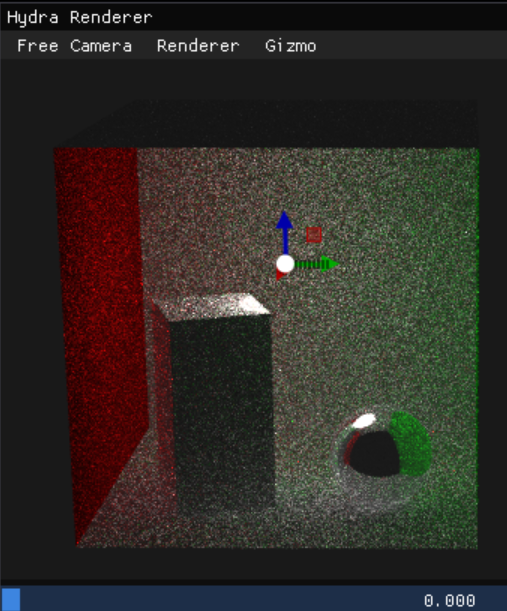
\includegraphics[width=\textwidth]{image-20260423205356335.png}
\caption{BRDF与MIS效果}
\end{subfigure}
\begin{subfigure}{0.32\textwidth}
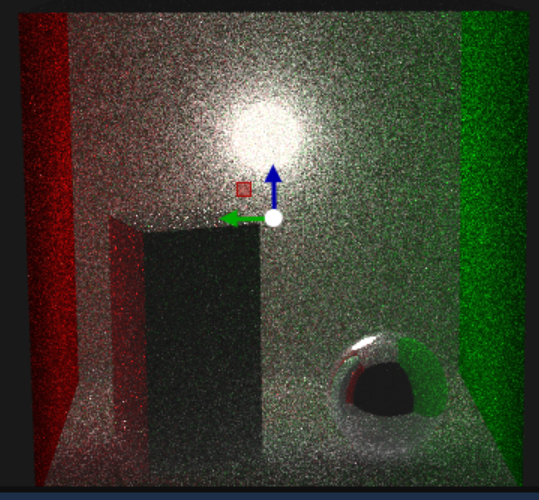
\includegraphics[width=\textwidth]{image-20260423213435685.png}
\caption{其他角度}
\end{subfigure}
\begin{subfigure}{0.32\textwidth}
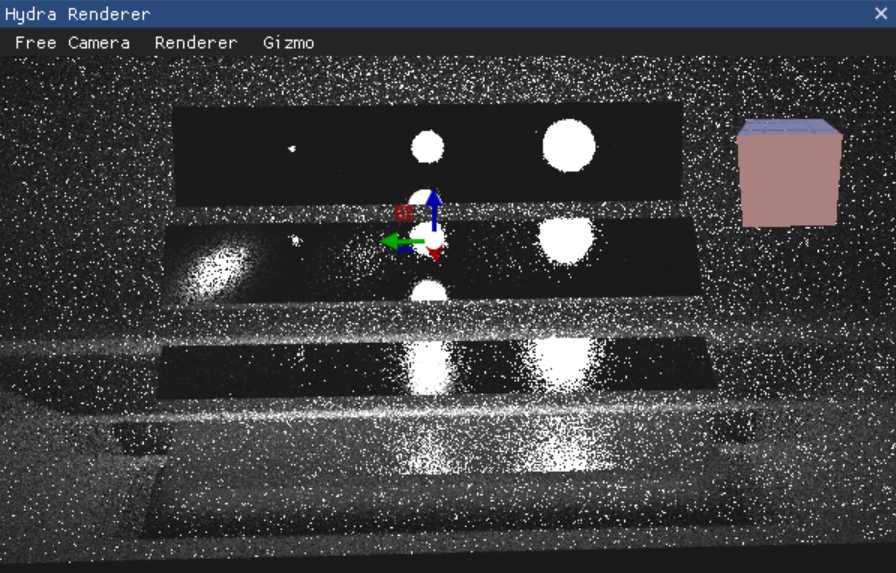
\includegraphics[width=\textwidth]{image-20260423215441926.png}
\caption{MIS效果}
\end{subfigure}
\caption{BRDF模型与MIS效果对比}
\end{figure}

\begin{figure}[H]
\centering
\begin{subfigure}{0.32\textwidth}
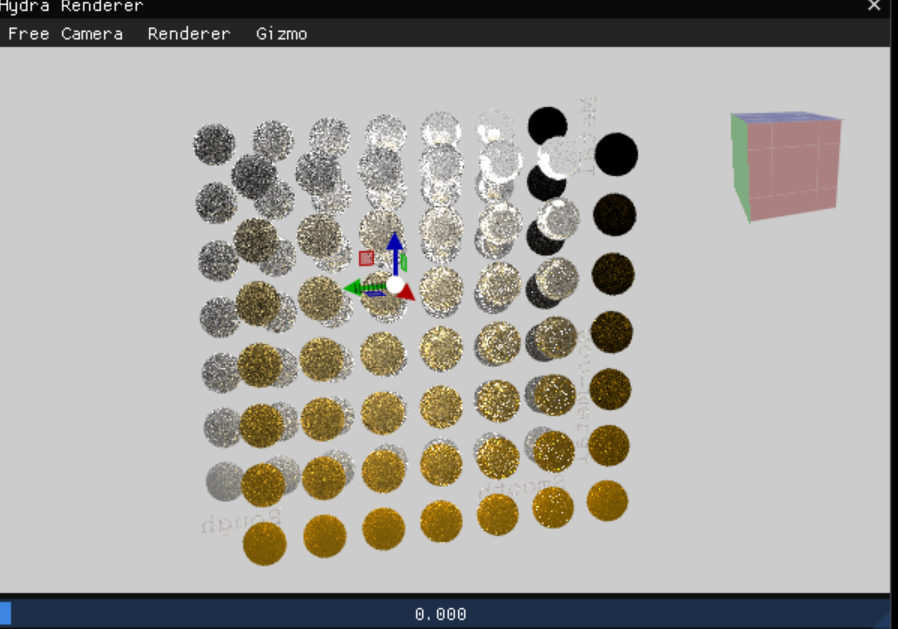
\includegraphics[width=\textwidth]{image-20260423215759151.png}
\caption{Sphere diffuse 0.8}
\end{subfigure}
\begin{subfigure}{0.32\textwidth}
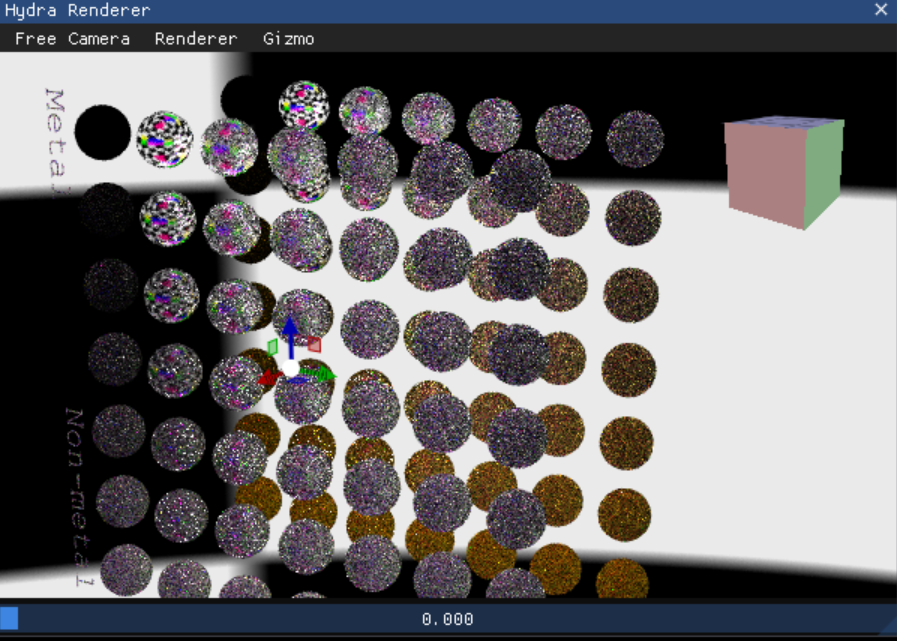
\includegraphics[width=\textwidth]{image-20260423221931131.png}
\caption{测试纹理}
\end{subfigure}
\begin{subfigure}{0.32\textwidth}
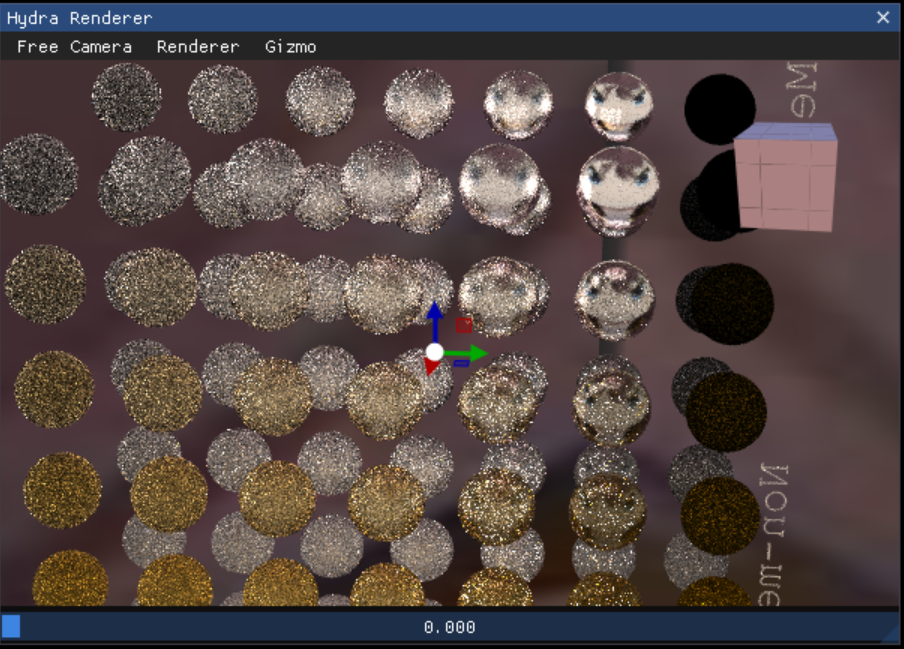
\includegraphics[width=\textwidth]{image-20260423222201159.png}
\caption{环境贴图反射}
\end{subfigure}
\caption{不同材质效果}
\end{figure}

\begin{figure}[H]
\centering
\begin{subfigure}{0.48\textwidth}
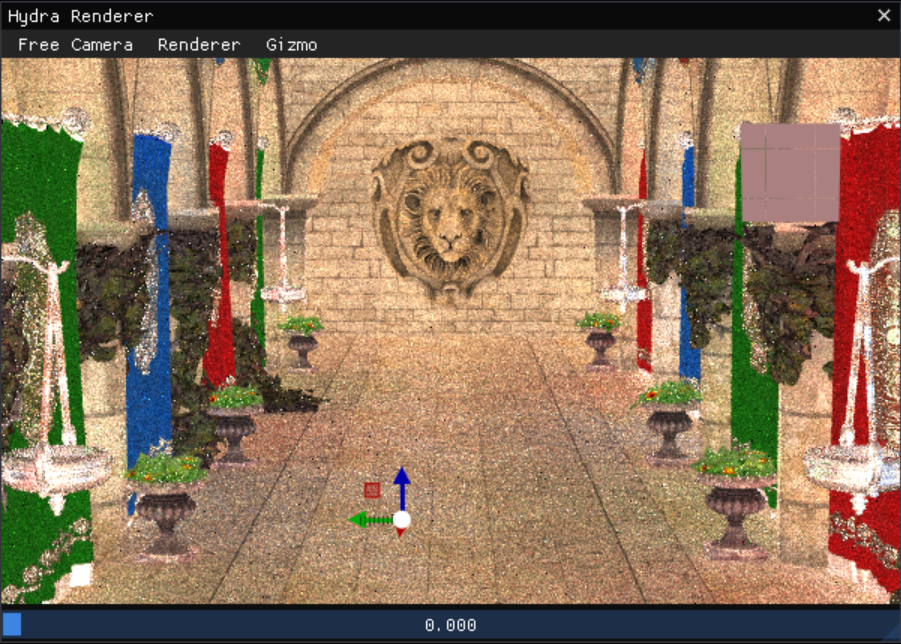
\includegraphics[width=\textwidth]{image-20260424200133735.png}
\caption{整体宏观效果}
\end{subfigure}
\begin{subfigure}{0.48\textwidth}
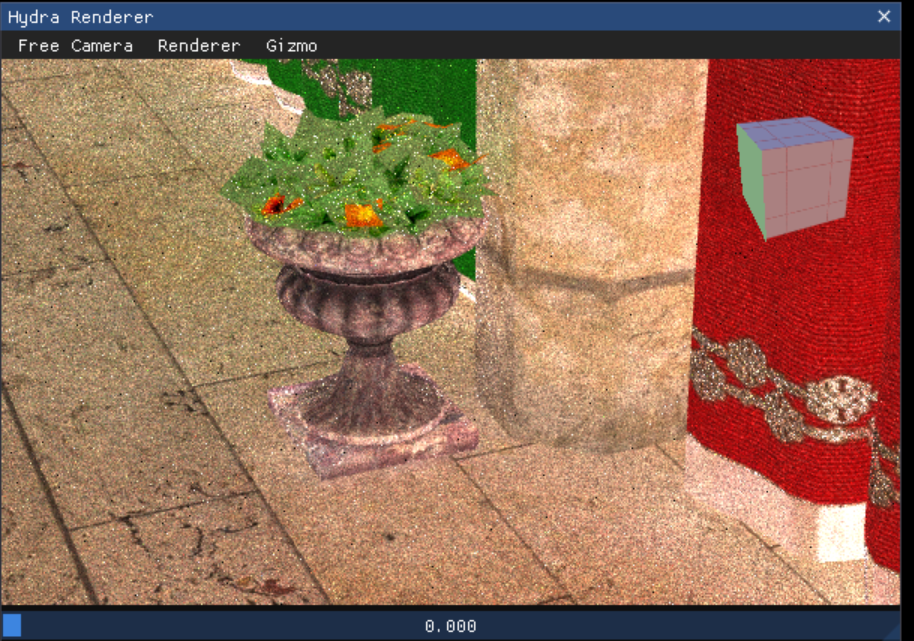
\includegraphics[width=\textwidth]{image-20260424195932209.png}
\caption{角落细节}
\end{subfigure}
\caption{Cornell Box场景效果}
\end{figure}

\begin{figure}[H]
\centering
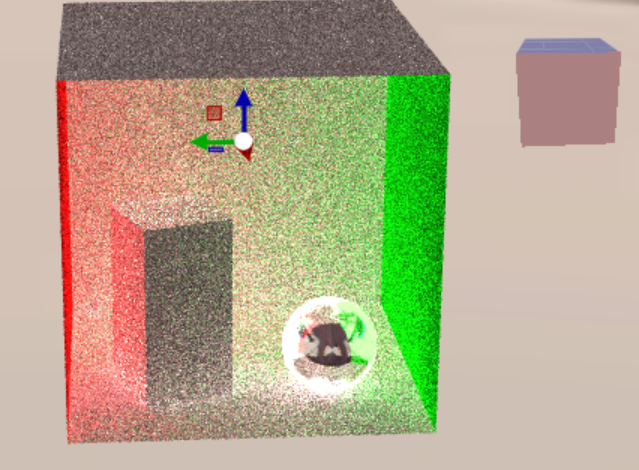
\includegraphics[width=0.5\textwidth]{image-20260424201413562.png}
\caption{Cornell Box自发光效果}
\end{figure}

\section{思考题}
\subsection{全面对比光栅 & 光追效果、时间等效果}
结合之前图片，发现光栅和光追两个对于同一场景效果很不一样，明显的是光追会有很多噪声，pdf计算的时候某些点没有计算到，虽然后续可以引入了G buffer辅助进一步游湖；
光追的渲染比光栅更慢，不用release根本慢的跑不了；

\subsection{修改参数，对比效果}






\end{CJK*}
\end{document}